\documentclass{standalone}
\usepackage{tikz}
\usetikzlibrary{patterns, positioning}
\usepackage[sfdefault]{ClearSans} %% option 'sfdefault' activates Clear Sans as the default text font
\usepackage[T1]{fontenc}

\begin{document}
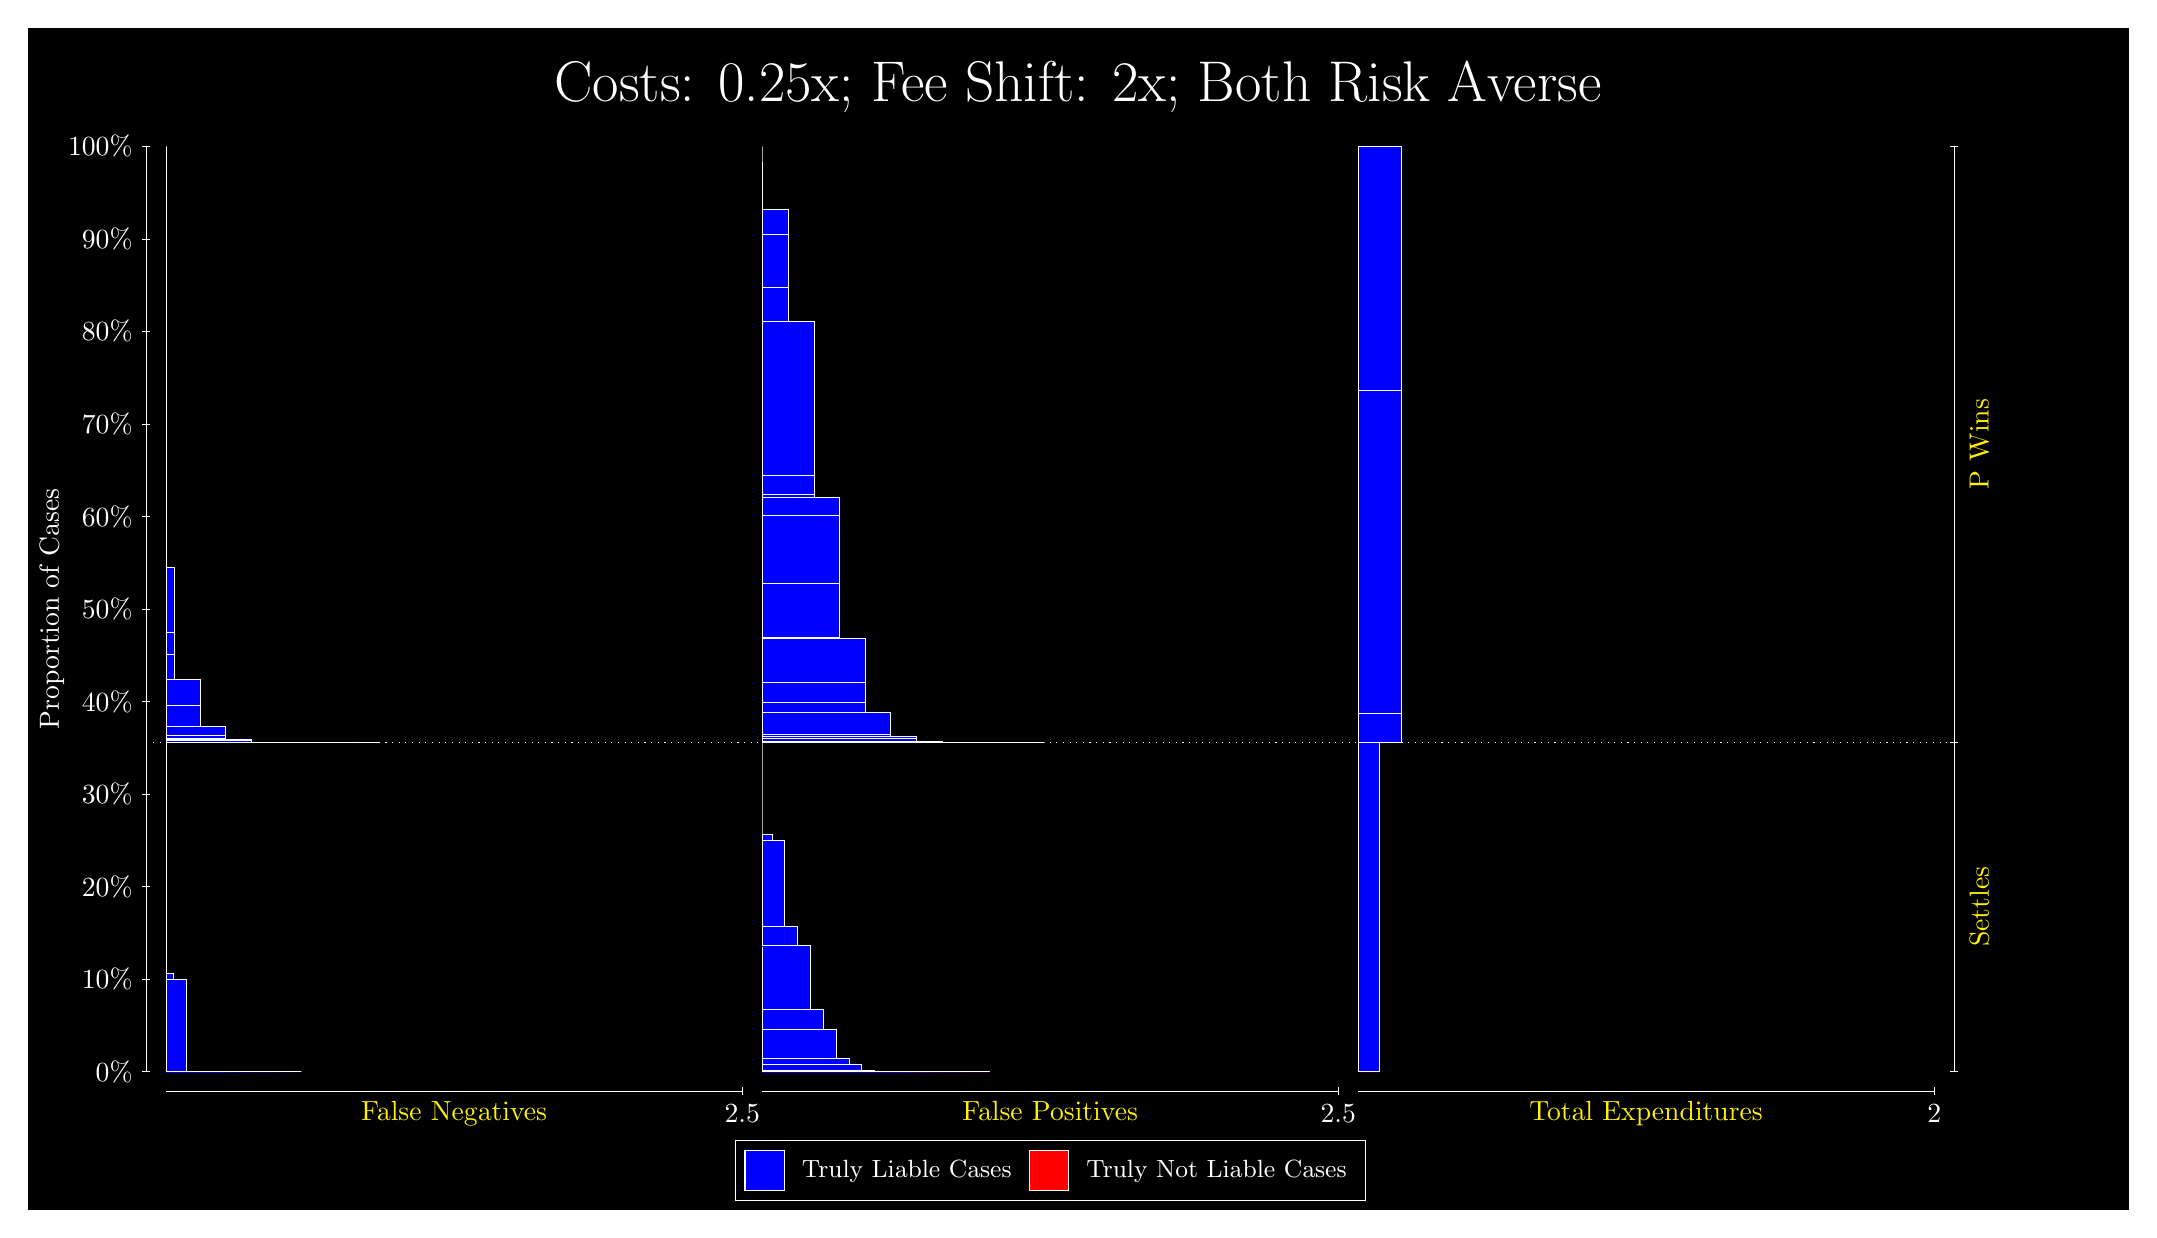
\begin{tikzpicture}
\draw[fill=black] (0,0) rectangle (26.667,15);
\draw[text=white] (0,13.5) rectangle (26.667,15) node[midway] {\huge Costs: 0.25x; Fee Shift: 2x; Both Risk Averse};
\draw[white, very thin] (1.5,1.75) -- (1.5,13.5);
\node[rotate=90, text=white, anchor=center] at (0.3, 7.625) {Proportion of Cases};
\draw[white, very thin] (1.45,1.75) -- (1.55,1.75);
\node[text=white, anchor=east] at (1.45, 1.75) {0\%};
\draw[white, very thin] (1.45,2.925) -- (1.55,2.925);
\node[text=white, anchor=east] at (1.45, 2.925) {10\%};
\draw[white, very thin] (1.45,4.1) -- (1.55,4.1);
\node[text=white, anchor=east] at (1.45, 4.1) {20\%};
\draw[white, very thin] (1.45,5.275) -- (1.55,5.275);
\node[text=white, anchor=east] at (1.45, 5.275) {30\%};
\draw[white, very thin] (1.45,6.45) -- (1.55,6.45);
\node[text=white, anchor=east] at (1.45, 6.45) {40\%};
\draw[white, very thin] (1.45,7.625) -- (1.55,7.625);
\node[text=white, anchor=east] at (1.45, 7.625) {50\%};
\draw[white, very thin] (1.45,8.8) -- (1.55,8.8);
\node[text=white, anchor=east] at (1.45, 8.8) {60\%};
\draw[white, very thin] (1.45,9.975) -- (1.55,9.975);
\node[text=white, anchor=east] at (1.45, 9.975) {70\%};
\draw[white, very thin] (1.45,11.15) -- (1.55,11.15);
\node[text=white, anchor=east] at (1.45, 11.15) {80\%};
\draw[white, very thin] (1.45,12.325) -- (1.55,12.325);
\node[text=white, anchor=east] at (1.45, 12.325) {90\%};
\draw[white, very thin] (1.45,13.5) -- (1.55,13.5);
\node[text=white, anchor=east] at (1.45, 13.5) {100\%};

\draw[white, very thin] (24.457,1.75) -- (24.457,13.5);
\draw[white, very thin] (24.407,1.75) -- (24.507,1.75);
\node[anchor=west] at (24.407, 1.75) {};
\draw[white, very thin] (24.407,5.9343) -- (24.507,5.9343);
\node[anchor=west] at (24.407, 5.9343) {};
\draw[white, very thin] (24.407,13.5) -- (24.507,13.5);
\node[anchor=west] at (24.407, 13.5) {};

\draw[white, very thin, fill=blue] (1.75,1.75) rectangle (3.4699,1.75);
\draw[white, very thin, fill=blue] (1.75,1.75) rectangle (3.1447,1.75);
\draw[white, very thin, fill=blue] (1.75,1.75) rectangle (2.8194,1.75);
\draw[white, very thin, fill=blue] (1.75,1.75) rectangle (2.738,1.75);
\draw[white, very thin, fill=blue] (1.75,1.75) rectangle (2.4941,1.7502);
\draw[white, very thin, fill=blue] (1.75,1.7502) rectangle (2.4128,1.7502);
\draw[white, very thin, fill=blue] (1.75,1.7502) rectangle (2.1688,1.757);
\draw[white, very thin, fill=blue] (1.75,1.757) rectangle (2.0875,1.757);
\draw[white, very thin, fill=blue] (1.75,1.757) rectangle (2.0062,2.9214);
\draw[white, very thin, fill=blue] (1.75,2.9214) rectangle (1.8435,2.9942);
\draw[white, very thin, fill=blue] (1.75,2.9942) rectangle (1.7622,2.9943);
\draw[white, very thin, fill=red] (1.75,2.9943) rectangle (1.75,2.9943);
\draw[white, very thin, fill=blue] (1.75,2.9943) rectangle (1.75,5.9343);
\draw[white, very thin, fill=blue] (1.75,5.9343) rectangle (4.458,5.9343);
\draw[white, very thin, fill=blue] (1.75,5.9343) rectangle (4.1327,5.9343);
\draw[white, very thin, fill=blue] (1.75,5.9343) rectangle (3.8074,5.9343);
\draw[white, very thin, fill=blue] (1.75,5.9343) rectangle (3.8074,5.9343);
\draw[white, very thin, fill=blue] (1.75,5.9343) rectangle (3.4821,5.9344);
\draw[white, very thin, fill=blue] (1.75,5.9344) rectangle (3.4821,5.9345);
\draw[white, very thin, fill=blue] (1.75,5.9345) rectangle (3.1568,5.9345);
\draw[white, very thin, fill=blue] (1.75,5.9345) rectangle (3.1568,5.9363);
\draw[white, very thin, fill=blue] (1.75,5.9363) rectangle (3.1568,5.9374);
\draw[white, very thin, fill=blue] (1.75,5.9374) rectangle (2.8316,5.9509);
\draw[white, very thin, fill=blue] (1.75,5.9509) rectangle (2.8316,5.9671);
\draw[white, very thin, fill=blue] (1.75,5.9671) rectangle (2.5063,5.9823);
\draw[white, very thin, fill=blue] (1.75,5.9823) rectangle (2.5063,6.0237);
\draw[white, very thin, fill=blue] (1.75,6.0237) rectangle (2.5063,6.1358);
\draw[white, very thin, fill=blue] (1.75,6.1358) rectangle (2.181,6.4032);
\draw[white, very thin, fill=blue] (1.75,6.4032) rectangle (2.181,6.7357);
\draw[white, very thin, fill=blue] (1.75,6.7357) rectangle (1.8557,7.05);
\draw[white, very thin, fill=blue] (1.75,7.05) rectangle (1.8557,7.3249);
\draw[white, very thin, fill=blue] (1.75,7.3249) rectangle (1.8557,8.1512);
\draw[white, very thin, fill=red] (1.75,8.1512) rectangle (1.75,8.1512);
\draw[white, very thin, fill=blue] (1.75,8.1512) rectangle (1.75,13.5);
\draw[white, very thin, fill=red] (9.3189,1.75) rectangle (12.21,1.75);
\draw[white, very thin, fill=blue] (9.3189,1.75) rectangle (12.21,1.75);
\draw[white, very thin, fill=blue] (9.3189,1.75) rectangle (11.885,1.75);
\draw[white, very thin, fill=blue] (9.3189,1.75) rectangle (11.559,1.75);
\draw[white, very thin, fill=red] (9.3189,1.75) rectangle (11.478,1.75);
\draw[white, very thin, fill=blue] (9.3189,1.75) rectangle (11.478,1.75);
\draw[white, very thin, fill=blue] (9.3189,1.75) rectangle (11.234,1.7502);
\draw[white, very thin, fill=blue] (9.3189,1.7502) rectangle (11.153,1.7502);
\draw[white, very thin, fill=blue] (9.3189,1.7502) rectangle (10.909,1.757);
\draw[white, very thin, fill=blue] (9.3189,1.757) rectangle (10.827,1.757);
\draw[white, very thin, fill=red] (9.3189,1.757) rectangle (10.746,1.757);
\draw[white, very thin, fill=blue] (9.3189,1.757) rectangle (10.746,1.7675);
\draw[white, very thin, fill=blue] (9.3189,1.7675) rectangle (10.583,1.8455);
\draw[white, very thin, fill=blue] (9.3189,1.8455) rectangle (10.502,1.8455);
\draw[white, very thin, fill=blue] (9.3189,1.8455) rectangle (10.421,1.9236);
\draw[white, very thin, fill=blue] (9.3189,1.9236) rectangle (10.258,2.2859);
\draw[white, very thin, fill=blue] (9.3189,2.2859) rectangle (10.177,2.2864);
\draw[white, very thin, fill=blue] (9.3189,2.2864) rectangle (10.095,2.5379);
\draw[white, very thin, fill=blue] (9.3189,2.5379) rectangle (9.9328,3.3481);
\draw[white, very thin, fill=blue] (9.3189,3.3481) rectangle (9.8515,3.3486);
\draw[white, very thin, fill=blue] (9.3189,3.3486) rectangle (9.7702,3.5991);
\draw[white, very thin, fill=blue] (9.3189,3.5991) rectangle (9.6076,4.69);
\draw[white, very thin, fill=blue] (9.3189,4.69) rectangle (9.5262,4.6901);
\draw[white, very thin, fill=blue] (9.3189,4.6901) rectangle (9.4449,4.7629);
\draw[white, very thin, fill=blue] (9.3189,4.7629) rectangle (9.3189,5.9343);
\draw[white, very thin, fill=red] (9.3189,5.9343) rectangle (12.905,5.9343);
\draw[white, very thin, fill=blue] (9.3189,5.9343) rectangle (12.905,5.9343);
\draw[white, very thin, fill=red] (9.3189,5.9343) rectangle (12.58,5.9343);
\draw[white, very thin, fill=blue] (9.3189,5.9343) rectangle (12.58,5.9343);
\draw[white, very thin, fill=red] (9.3189,5.9343) rectangle (12.255,5.9343);
\draw[white, very thin, fill=blue] (9.3189,5.9343) rectangle (12.255,5.9343);
\draw[white, very thin, fill=blue] (9.3189,5.9343) rectangle (11.929,5.9344);
\draw[white, very thin, fill=blue] (9.3189,5.9344) rectangle (11.929,5.9346);
\draw[white, very thin, fill=red] (9.3189,5.9346) rectangle (11.929,5.9346);
\draw[white, very thin, fill=blue] (9.3189,5.9346) rectangle (11.929,5.9349);
\draw[white, very thin, fill=blue] (9.3189,5.9349) rectangle (11.604,5.9374);
\draw[white, very thin, fill=red] (9.3189,5.9374) rectangle (11.604,5.9374);
\draw[white, very thin, fill=blue] (9.3189,5.9374) rectangle (11.604,5.9409);
\draw[white, very thin, fill=blue] (9.3189,5.9409) rectangle (11.604,5.9425);
\draw[white, very thin, fill=blue] (9.3189,5.9425) rectangle (11.279,5.9799);
\draw[white, very thin, fill=red] (9.3189,5.9799) rectangle (11.279,5.9799);
\draw[white, very thin, fill=blue] (9.3189,5.9799) rectangle (11.279,6.0038);
\draw[white, very thin, fill=blue] (9.3189,6.0038) rectangle (10.953,6.0349);
\draw[white, very thin, fill=red] (9.3189,6.0349) rectangle (10.953,6.0349);
\draw[white, very thin, fill=blue] (9.3189,6.0349) rectangle (10.953,6.3099);
\draw[white, very thin, fill=blue] (9.3189,6.3099) rectangle (10.628,6.4434);
\draw[white, very thin, fill=blue] (9.3189,6.4434) rectangle (10.628,6.6914);
\draw[white, very thin, fill=red] (9.3189,6.6914) rectangle (10.628,6.6914);
\draw[white, very thin, fill=blue] (9.3189,6.6914) rectangle (10.628,7.2462);
\draw[white, very thin, fill=blue] (9.3189,7.2462) rectangle (10.303,7.2673);
\draw[white, very thin, fill=blue] (9.3189,7.2673) rectangle (10.303,7.9566);
\draw[white, very thin, fill=red] (9.3189,7.9566) rectangle (10.303,7.9566);
\draw[white, very thin, fill=blue] (9.3189,7.9566) rectangle (10.303,8.8174);
\draw[white, very thin, fill=blue] (9.3189,8.8174) rectangle (10.303,9.0474);
\draw[white, very thin, fill=blue] (9.3189,9.0474) rectangle (9.9776,9.0779);
\draw[white, very thin, fill=blue] (9.3189,9.0779) rectangle (9.9776,9.3216);
\draw[white, very thin, fill=red] (9.3189,9.3216) rectangle (9.9776,9.3216);
\draw[white, very thin, fill=blue] (9.3189,9.3216) rectangle (9.9776,11.283);
\draw[white, very thin, fill=blue] (9.3189,11.283) rectangle (9.6523,11.712);
\draw[white, very thin, fill=blue] (9.3189,11.712) rectangle (9.6523,12.388);
\draw[white, very thin, fill=blue] (9.3189,12.388) rectangle (9.6523,12.699);
\draw[white, very thin, fill=blue] (9.3189,12.699) rectangle (9.327,13.299);
\draw[white, very thin, fill=blue] (9.3189,13.299) rectangle (9.3189,13.5);
\draw[white, very thin, fill=red] (16.888,1.75) rectangle (17.162,1.75);
\draw[white, very thin, fill=blue] (16.888,1.75) rectangle (17.162,5.9343);
\draw[white, very thin, fill=red] (16.888,5.9343) rectangle (17.437,5.9343);
\draw[white, very thin, fill=blue] (16.888,5.9343) rectangle (17.437,6.2974);
\draw[white, very thin, fill=red] (16.888,6.2974) rectangle (17.437,6.2974);
\draw[white, very thin, fill=blue] (16.888,6.2974) rectangle (17.437,10.4);
\draw[white, very thin, fill=red] (16.888,10.4) rectangle (17.437,10.4);
\draw[white, very thin, fill=blue] (16.888,10.4) rectangle (17.437,13.5);
\draw[white, dotted] (1.5,5.9343) -- (24.457,5.9343);
\draw[white, very thin] (1.75,1.5) -- (9.0689,1.5);
\node[text=yellow, anchor=north] at (5.4094, 1.5) {False Negatives};
\draw[white, very thin] (9.0689,1.45) -- (9.0689,1.55);
\node[text=white, anchor=north] at (9.0689, 1.45) {2.5};

\draw[white, very thin] (9.3189,1.5) -- (16.638,1.5);
\node[text=yellow, anchor=north] at (12.978, 1.5) {False Positives};
\draw[white, very thin] (16.638,1.45) -- (16.638,1.55);
\node[text=white, anchor=north] at (16.638, 1.45) {2.5};

\draw[white, very thin] (16.888,1.5) -- (24.207,1.5);
\node[text=yellow, anchor=north] at (20.547, 1.5) {Total Expenditures};
\draw[white, very thin] (24.207,1.45) -- (24.207,1.55);
\node[text=white, anchor=north] at (24.207, 1.45) {2};

\node[text=yellow, centered, rotate=90] at (24.777, 3.8422) {Settles};
\node[text=yellow, centered, rotate=90] at (24.777, 9.7172) {P Wins};

\draw (12.978300999999998,1.5) node[draw=none] (baseCoordinate) {};
\begin{scope}[align=center]
        \matrix[scale=0.5, draw=white, below=0.5cm of baseCoordinate, nodes={draw}, column sep=0.1cm]{
            \node[rectangle, draw, minimum width=0.5cm, minimum height=0.5cm, fill=blue] {}; &
            \node[draw=none, font=\small, text=white] (B) {Truly Liable Cases}; &
            \node[rectangle, draw, minimum width=0.5cm, minimum height=0.5cm, fill=red] {}; &
            \node[draw=none, font=\small, text=white] (B) {Truly Not Liable Cases}; \\
            };
\end{scope}

\end{tikzpicture}
\end{document}